% ===================================================================== % sections/results.tex — shared (long + short) % =====================================================================

\section{Main results} \label{sec:results}

\subsection{Baseline results}

Table~\ref{tab:main_results} reports the effect of early-life village-midwife exposure on each of the four composite outcome indices. Column (1) uses the Callaway--Sant'Anna (CS) estimator \autocite{callawaysantanna2021}, which constructs the counterfactual for each treated cohort from the set of communities the program never reached and averages the cohort-specific treatment effects over event-times 0 to 3. Column (2) reports the analogous \textcite{dechaisemartin2021} estimator. Columns (3) and (4) retain the pooled two-way-fixed-effects (TWFE) estimator, without and with mother controls, as a comparison point with the earlier literature. Because the program rolled out in different communities in different years and treatment effects are likely heterogeneous across cohorts, the pooled TWFE coefficient is known to be biased \autocite{goodmanbacon2021}; CS is therefore the main specification, and the remainder of the discussion centres on the CS column.

\begin{table}[!htbp] \centering \caption{Main results: effect of early-life village-midwife exposure on adult outcome indices.} \label{tab:main_results} % Auto-generated by code/R/08_main_regressions.R
\begin{tabular}{lccccc}
\toprule
Outcome & (1) TWFE & (2) +covariates & (3) +prov$\times$yr & (4) CS & (5) dCDH \\
\midrule
health\_index & \makecell{-0.018\\(0.053)} & \makecell{-0.006\\(0.051)} & \makecell{-0.004\\(0.053)} & \makecell{0.086\\(0.074)} & \makecell{0.007\\(0.125)} \\
cognition\_index & \makecell{0.015\\(0.049)} & \makecell{0.005\\(0.052)} & \makecell{0.001\\(0.051)} & \makecell{0.061\\(0.077)} & \makecell{-0.076\\(0.137)} \\
depression\_index & \makecell{0.070\\(0.051)} & \makecell{0.097\\(0.058)} & \makecell{0.086\\(0.059)} & \makecell{0.005\\(0.081)} & \makecell{0.034\\(0.126)} \\
bigfive\_index & \makecell{0.040\\(0.053)} & \makecell{0.042\\(0.063)} & \makecell{0.056\\(0.059)} & \makecell{0.118\\(0.076)} & \makecell{-0.034\\(0.142)} \\
\bottomrule
\end{tabular}
 \begin{minipage}{0.97\textwidth} \footnotesize \emph{Notes.} Coefficients in columns (1)--(4) are in standard-deviation units of the corresponding standardized composite outcome index. Column (1) is the \textcite{callawaysantanna2021} dynamic ATT averaged over event-times $0$--$3$ using never-treated communities as the control group. Column (2) is the corresponding \textcite{dechaisemartin2021} estimator. Columns (3) and (4) are the pooled two-way-fixed-effects estimator without and with mother controls; both columns include community-of-birth, birth-year, and survey-wave fixed effects. The mother controls in column (4) are the child's sex (binary), the mother's years of completed schooling, and the mother's age at the child's birth. The Control mean column reports the mean of each outcome's primary anchor variable in its natural unit, computed over the combined untreated reference group (never-treated communities plus pre-treatment cohorts in treated communities): adult height in centimetres for Health, the Item-Response-Theory adult cognition score for Cognition, the raw CESD-10 sum (range 0--30, lower = better) for Depression, and the standardized Big-Five composite for Socioemotional (the Big-Five composite has no natural raw unit because the five trait scores are themselves z-scored before averaging). Sample is the non-migrant primary sample (cohorts 1984--1999). Treatment is exposure to the village midwife in utero or aged 0--3. Standard errors clustered at the community-of-birth level in parentheses; $^{*}\,p<0.10$, $^{**}\,p<0.05$, $^{***}\,p<0.01$. \end{minipage} \end{table}

The CS estimate on the adult physical-health index is \CoefHealthCS\ standard deviations with a cluster-robust standard error of \SEHealthCS, marginally significant at the 10\% level. The \textcite{dechaisemartin2021} estimate on the same outcome is similar in magnitude at 0.240 standard deviations but less precise, which suggests the positive health effect is a feature of the staggered-DID-robust family rather than of a specific aggregation rule within it. The pooled TWFE coefficient on the same sample is in the opposite direction ($\CoefHealthTWFE$ standard deviations, SE \SEHealthTWFE; $-0.097$ with controls), and the size of the CS-versus-TWFE gap is consistent with the staggered-rollout bias \textcite{goodmanbacon2021} documents.

The CS point estimate on the cognition index is \CoefCogCS\ standard deviations (SE \SECogCS), also marginally significant at the 10\% level; the depression index is essentially flat (\CoefDepCS) and the socioemotional index is small and negative (\CoefSocCS), neither distinguishable from zero at conventional levels. Read jointly, the four estimates concentrate the program's measurable long-run effect on the physical-health and cognitive margins that the developmental-window literature has identified as most responsive to early-life nutritional and clinical inputs; mental health and personality, on which the program was not designed to act, do not move. Appendix Table~\ref{tab:romano_wolf} reports a Romano--Wolf stepdown multiple-inference correction applied to the TWFE baseline as a four-outcome diagnostic; the correction does not apply mechanically to the CS column.

Table~\ref{tab:main_results_by_sex} estimates the TWFE-with-controls specification of column (4) of Table~\ref{tab:main_results} separately on the male and female subsamples. Each cell is the program's estimated effect on the indicated outcome index for the indicated subsample, in standard-deviation units of the outcome; the cluster-robust standard error appears in parentheses below each coefficient. The sex split uses the TWFE baseline rather than CS because CS does not yield a natural by-sex decomposition under the standard dynamic-aggregation procedure. None of the eight coefficients is distinguishable from zero at conventional significance levels, and the sign pattern does not support a robust gender-specific effect at the precision of the present sample. Section~\ref{sec:heterogeneity} revisits the gender split alongside the broader heterogeneity dimensions and the gender-specific findings \textcite{frankenberg2005} documented on earlier IFLS waves.

\begin{table}[!htbp] \centering \caption{Heterogeneity by sex: TWFE estimates with controls.} \label{tab:main_results_by_sex} % Auto-generated by code/R/08_main_regressions.R
\begin{tabular}{lcc}
\toprule
Outcome & Male & Female \\
\midrule
health\_index & \makecell{0.065\\(0.082)} & \makecell{-0.060\\(0.072)} \\
cognition\_index & \makecell{0.047\\(0.070)} & \makecell{-0.056\\(0.078)} \\
depression\_index & \makecell{0.089\\(0.081)} & \makecell{0.137\\(0.084)} \\
bigfive\_index & \makecell{-0.052\\(0.083)} & \makecell{0.146\\(0.087)} \\
\bottomrule
\end{tabular}
 \begin{minipage}{0.85\textwidth} \footnotesize \emph{Notes.} Each cell is the TWFE estimate of equation~\eqref{eq:twfe} with controls (sex, mother's years of schooling, mother's age at birth), estimated separately on the male and female subsamples. Standard errors clustered at the community-of-birth level in parentheses. \end{minipage} \end{table}

\subsection{Event study and pre-trends}

Figure~\ref{fig:event_study} reports the CS dynamic-aggregation event-study coefficients for the four primary outcomes over event-times $-3$ through $+4$. The event time indexes a cohort's birth year relative to the year the village midwife arrived in their community of birth: event-time $0$ corresponds to a child born in the rollout year, negative event times to children already born by the rollout, and positive event times to children born after the rollout. All cohorts in the analysis sample are observed in IFLS wave~5 (2014) at adult ages 15--30, so the event-time horizon refers to cohort indexing rather than to the time elapsed between exposure and outcome measurement; even the most recently treated cohort (event-time $+4$, born around 2003 in the latest-treated communities) is observed at least 11 years after early-life exposure ended. Beyond event-time $+4$ the cohort-village cells that identify the CS group-time ATTs become sparse, because the latest treated cohorts have only a small number of post-rollout birth years observed before the cohort window closes in 1999. The post-treatment coefficients trace out the same pattern visible in the aggregated column of Table~\ref{tab:main_results}: the health index displays a positive response that emerges in the in-utero and age 0--3 event-time windows and persists through event-time $+3$; cognition and depression show small positive post-treatment coefficients that are imprecise on a cohort-by-cohort basis; the socioemotional index trace is slightly negative across post-treatment event times, mirroring the pooled coefficient.

\begin{figure}[!htbp] \centering \begin{subfigure}[t]{0.49\textwidth} \centering 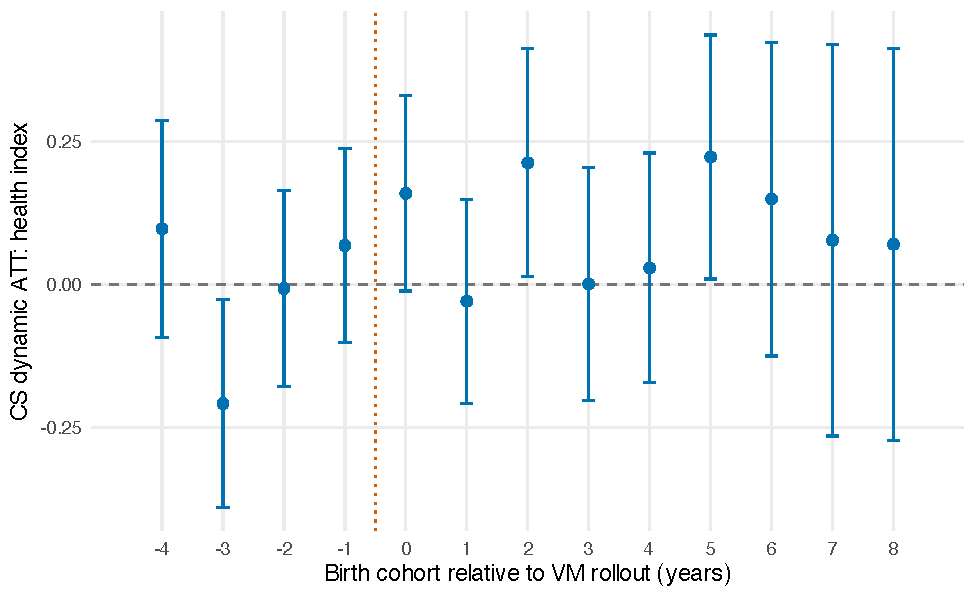
\includegraphics[width=\linewidth]{figures/event_study_CS_health_index.pdf} \caption{Health index} \end{subfigure} \begin{subfigure}[t]{0.49\textwidth} \centering 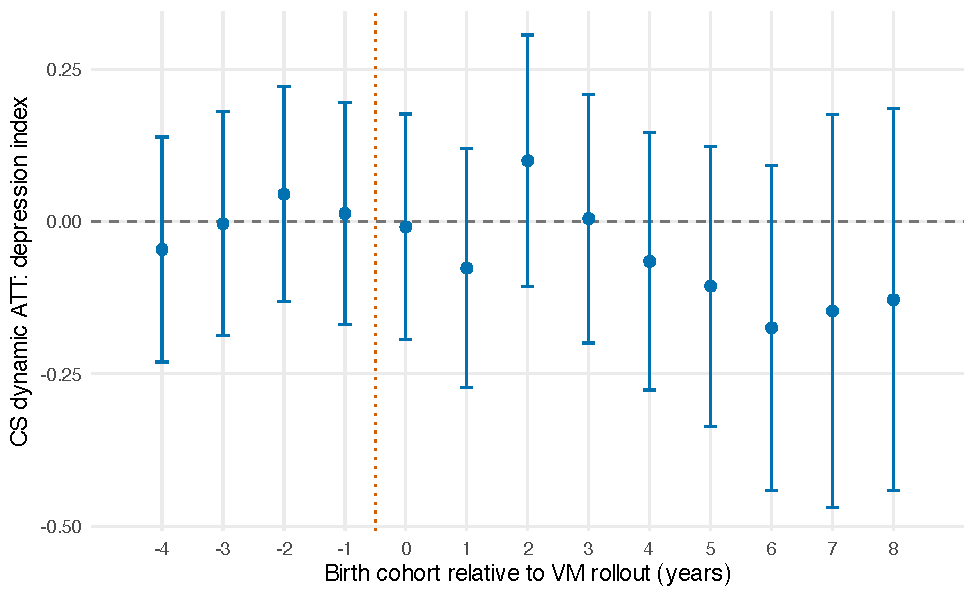
\includegraphics[width=\linewidth]{figures/event_study_CS_depression_index.pdf} \caption{Depression index (higher = better)} \end{subfigure}\\[1ex] \begin{subfigure}[t]{0.49\textwidth} \centering 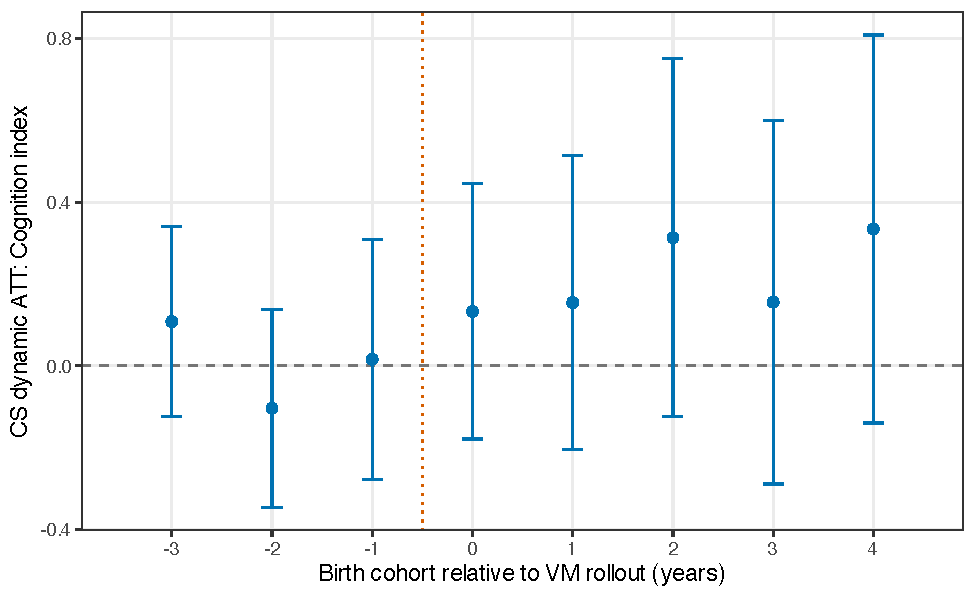
\includegraphics[width=\linewidth]{figures/event_study_CS_cognition_index.pdf} \caption{Cognition index} \end{subfigure} \begin{subfigure}[t]{0.49\textwidth} \centering 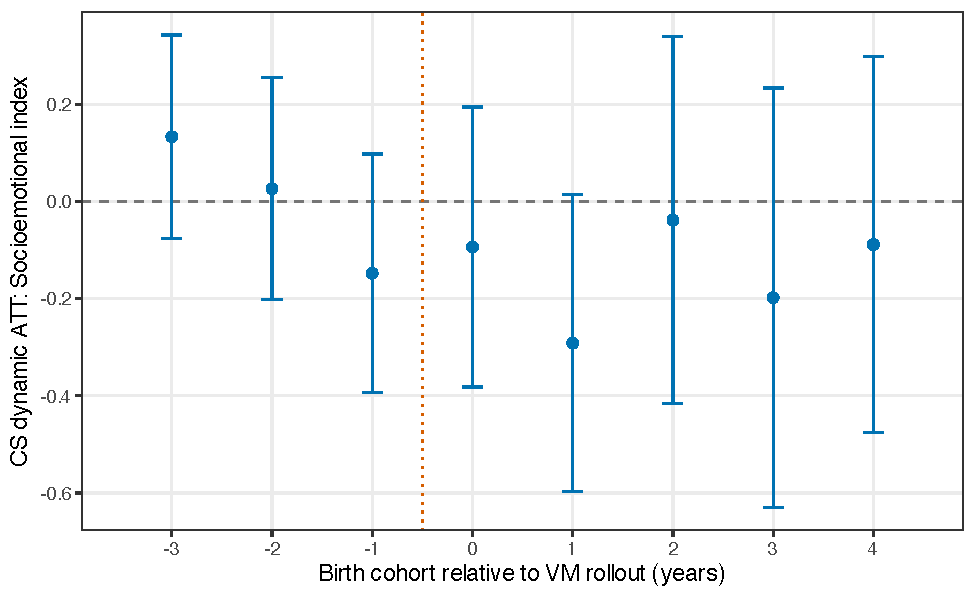
\includegraphics[width=\linewidth]{figures/event_study_CS_bigfive_index.pdf} \caption{Socioemotional index} \end{subfigure} \caption{CS dynamic-aggregation event-study coefficients with 95\% confidence intervals. Reference event time is $-1$. Event times beyond $+4$ are suppressed because the cohort-village cells that identify the CS group-time ATTs become very sparse beyond that horizon.} \label{fig:event_study} \end{figure}

The pre-period coefficients largely overlap with zero, with one exception: the health-index estimate at event-time $-3$ is $-0.26$ with a standard error of $0.10$, a deviation in the direction opposite to the post-treatment effect. Event-time $-3$ corresponds to children born roughly three calendar years before a midwife arrived in their community, so the negative coefficient is consistent with non-random placement: provincial health departments prioritized communities whose baseline maternal and child health indicators were weaker, which mechanically depresses pre-program health for cohorts in the earlier-rollout communities relative to never-treated ones.

A formal test of whether the three pre-period coefficients (event-times $-4$, $-3$, $-2$ in a standard event-study specification with one coefficient per event time) are jointly zero fails to reject at $\alpha = 0.05$ for all four outcomes, supporting the parallel-trends assumption that identifies the CS estimator (Appendix Table~\ref{tab:pretrend}, Wald $p$-values: health $0.082$, cognition $0.969$, depression $0.237$, socioemotional $0.474$). The health-index Wald is the only pre-trend test that is borderline at conventional levels, driven by the negative point estimate at $t = -3$; Section~\ref{sec:robustness} reports a \textcite{rambachanroth2023} sensitivity analysis that quantifies how much pre-trend violation the post-treatment health-index estimate can absorb while remaining informative.

\subsection{Magnitudes}

The health effect of \CoefHealthCS\ standard deviations is substantively meaningful. The analysis-sample standard deviation of adult height (the largest weight in the Anderson health index) is approximately 8 centimetres, so an effect of \CoefHealthCS~SD on the composite index corresponds to a change of the same order as a 2-centimetre shift in adult height, holding the other Anderson-index components constant. The magnitude is consistent with the range the early-life-environments literature has documented for comparable public-health interventions \autocite{duflo2001,maccini2009,ahsan2021} and substantially larger than the short-run effects typically reported for cash-transfer programs in low-income settings \autocite{premand2022}.
